\section{AR Viewer Version of the Space-Time Cube}\label{sec:ar-version}
The second presentation of the space-time cube that the users can opt for is meant for augmented reality viewers. This only works on
mobile devices with browsers that support WebXR. More about this is explained in \Cref{sec:webxr}.

After the AR version of the visualization is selected,
users are shown a circle indicator on their mobile devices and are given the option to place the cube according to their wishes by clicking on this circle.
After the cube is placed and the circle is gone, users can interact with the cube in a similar way as they interact with it in the browser version of the
cube. Now, instead of using the mouse and the keyboard, they move the mobile device around the cube, and come close or move away to zoom it in or out. They
have the toolbar for filtering options in order to show different information within the cube. This is mentioned in
\Cref{subsec:specifics-of-the-ar-version}.

\begin{figure}[hbt!]
    \centering
    \begin{subfigure}{.5\textwidth}
        \centering
        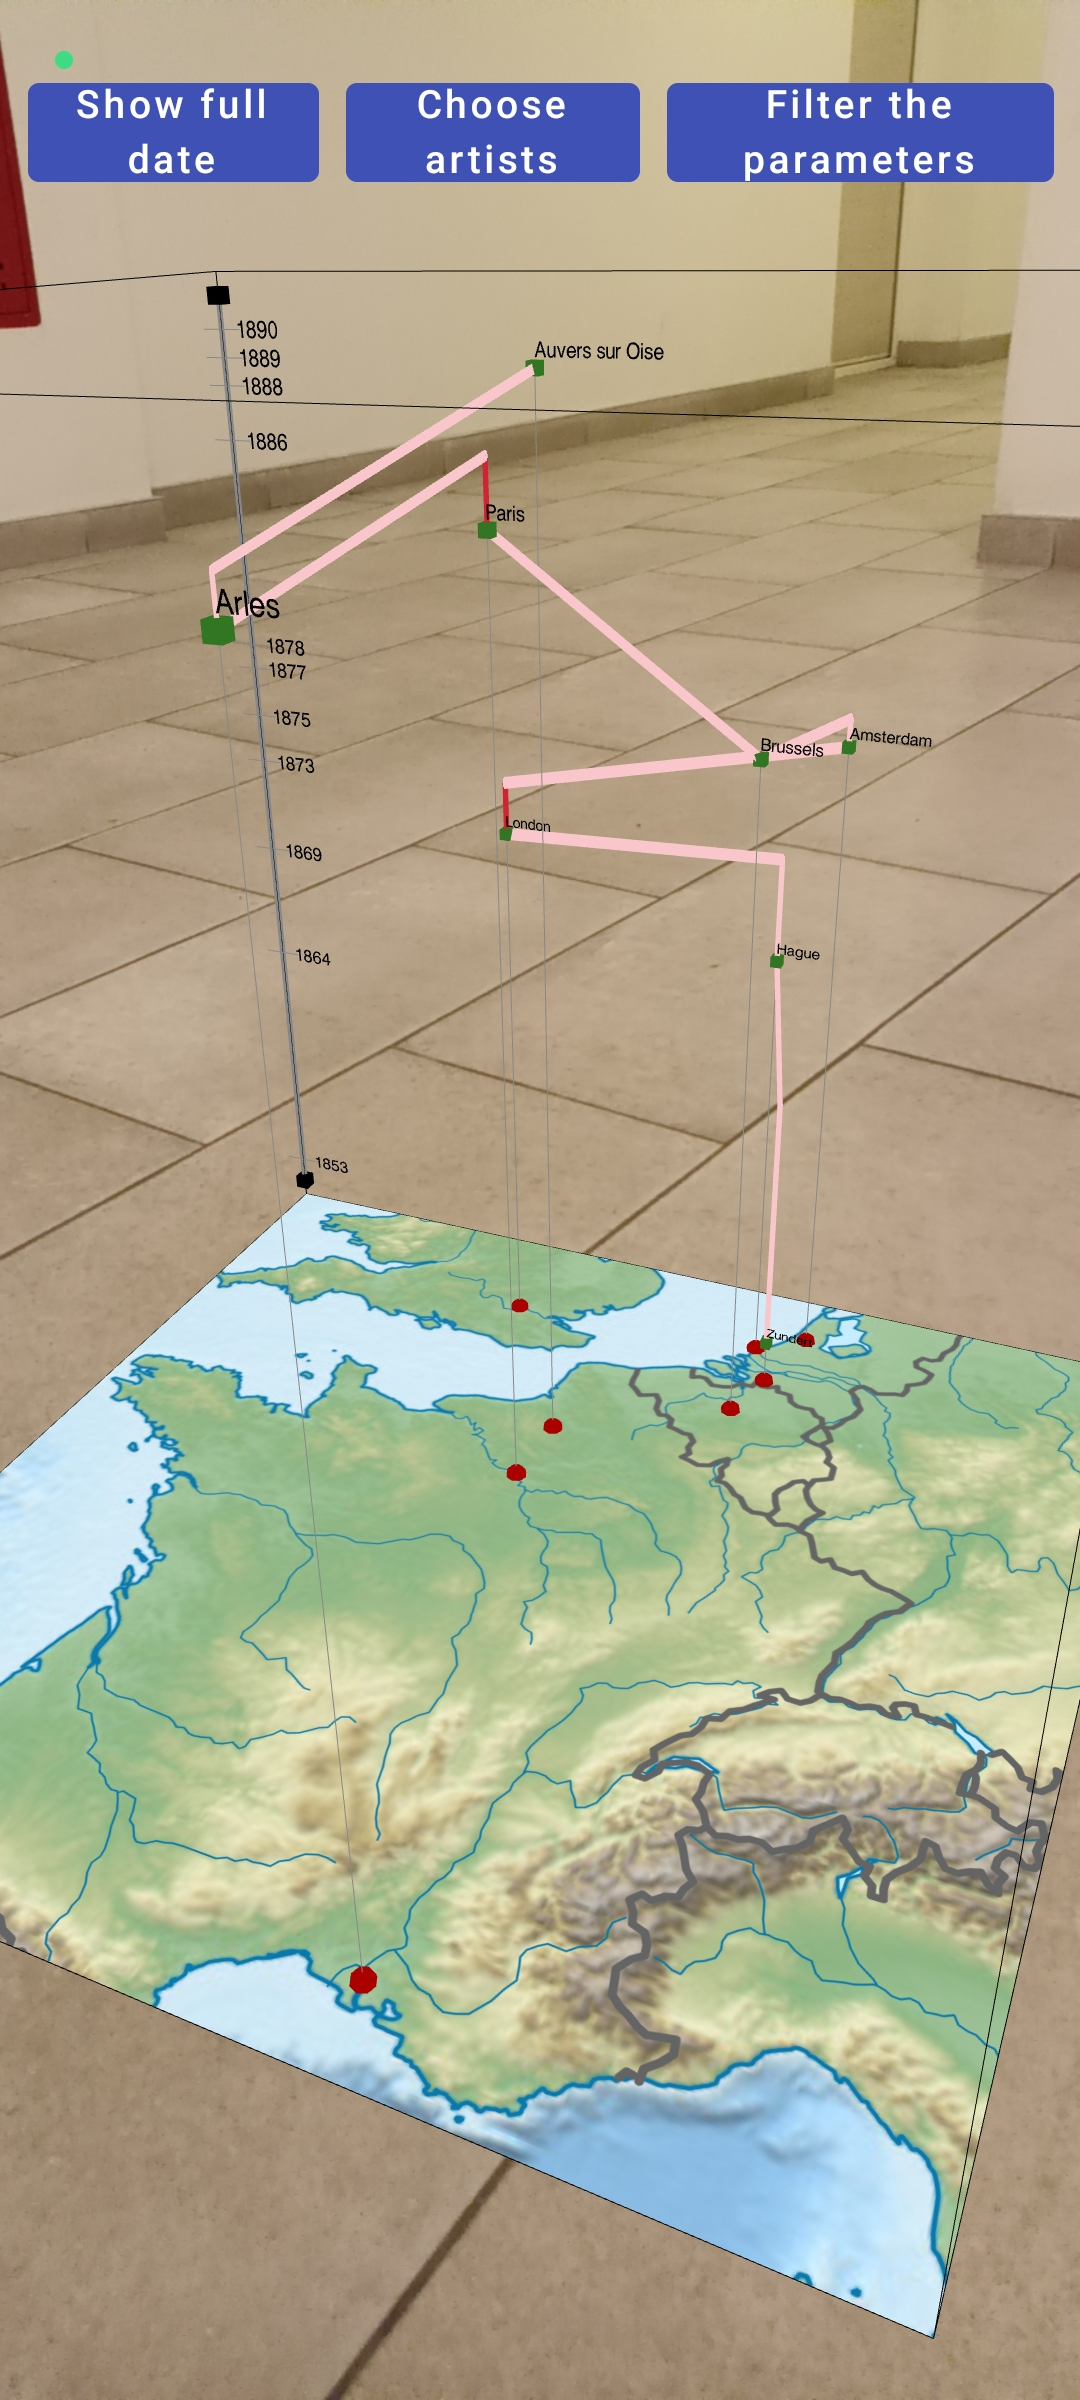
\includegraphics[width=0.7\linewidth]{graphics/3-implementation/ar1}
    \end{subfigure}%
    \begin{subfigure}{.5\textwidth}
        \centering
        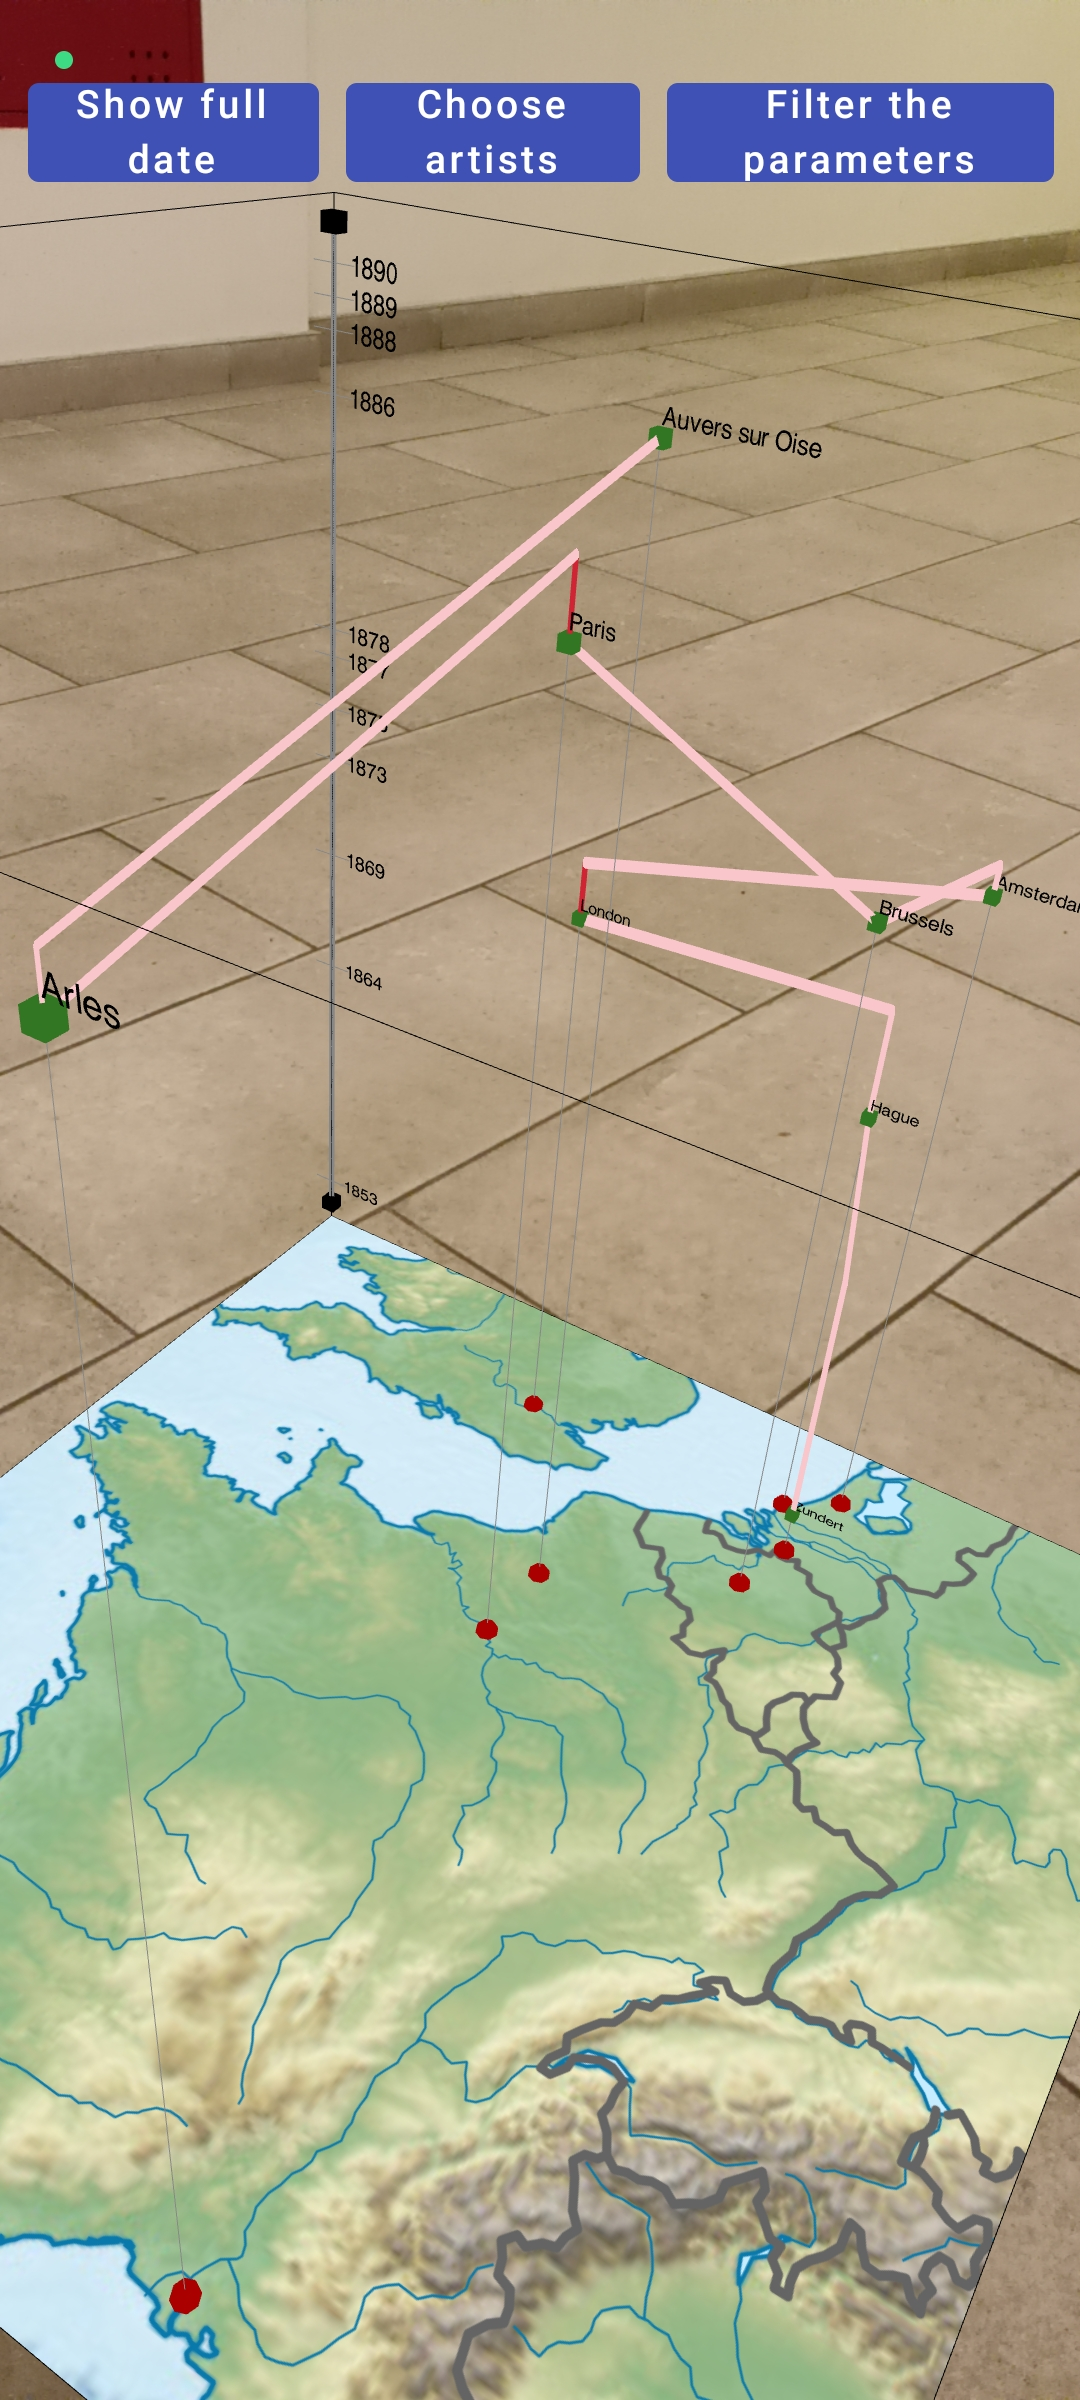
\includegraphics[width=0.7\linewidth]{graphics/3-implementation/ar3}
    \end{subfigure}
    \caption{AR visualization of the space-time cube}
    \label{fig:figure3.15}
\end{figure}

\subsection{Technical Features of the AR Version}\label{subsec:specifics-of-the-ar-version}

To place the cube in the real space, a concept that is similar to raycasting is applied -- \emph{hit test}. Hit test allows us to determine at which
point a mobile device looks at in the real space. Based on this point, a circle is drawn on the screen to show the user where the
cube will be placed when clicked on the screen. After clicking, the circle indicator disappears, the cube is drawn instead and fixed at that
position. The user can then interact with the cube by moving the mobile device around it.

Additionally, the AR takes over the control of the whole screen and draws the cube in full screen mode, whereas a UI (user interface) is needed
as well. Fortunately, this problem was noticed so an extension was defined in the WebXR specification which allows some DOM (Document Object Model)
element to be drawn for defining a UI on top of the AR screen. At the time of writing, this is the only way to show the UI in AR mode, but
unfortunately, not all viewers and browsers support it since the extension was added fairly recently. This leaves us with using Chrome on an Android
device for testing the AR experience.
